\chapter{Software}

\section{Introducción}
Se debe destacar que todo el desarrollo de software se basa exclusivamente en herramientas de software libre. La distribución Linux elegida para el sistema embebido se llama Angström. Ésta distribución es muy usada en aplicaciones que usan una Beagleboard y cuenta con una gran cantidad de bibliotecas implementadas en lenguaje C, que permiten una gran escalabilidad a la hora de incorporar nuevos periféricos en la aplicación.

\section{Arquitectura de Software}
\subsection{Descripción}
Un sistema linux en general se compone de diferentes partes que interactúan entre sí, formando capas ordenadas con distintos grados de abstracción respecto al hardware. Esto lo podemos apreciar en la (FIGURA) donde se muestra a grandes rasgos el sistema implementado. 

\begin{figure}[H]
\centering
  \begin{center}
  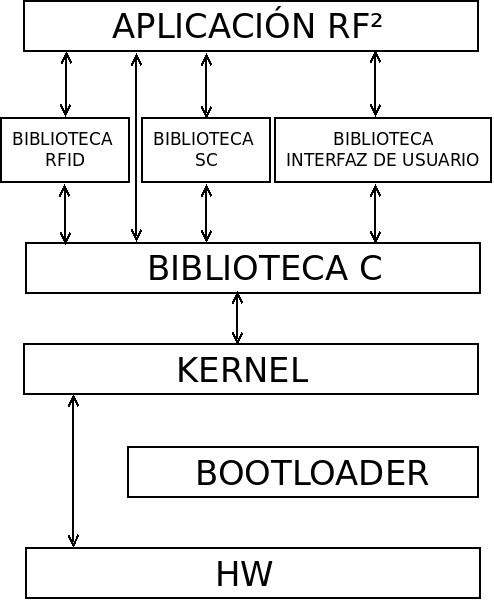
\includegraphics[scale=.4]{Imagenes/SW.jpg} 
  \end{center}
  \caption{Sistema ${RF^{2}}$}\label{Fig:HW} 
\end{figure}

El bootloader es la parte del sistema más primitiva y su función es la de cargar el kernel en memoria RAM para su ejecución. En general el bootloader se divide en dos etapas, la primera etapa del bootloader se encarga de buscar la segunda etapa del bootloader en particiones activas para luego cargarlo en RAM y ejecutarlo. La segunda etapa del bootloader se encarga de cargar una imagen comprimida del kernel en RAM y ejecutarlo. En este momento se descomprime el kernel y se cede el control al kernel.
El kernel se encarga a grandes rasgos de habilitar interrupciones, configurar la memoria y montar un sistema de archivos primitivo que permite a su vez cargar los módulos necesarios para la interfáz con periféricos. Luego se monta el verdadero sistema de archivos (fileSystem). En este nuevo sistema de archivos es donde se instalarán diferentes programas y bibliotecas para una correcta ejecución de nuestra aplicación.
En funcionamiento toda la comunicación con periféricos se realiza a través del kernel que es la parte más cercana al hardware.
Cada vez que ejecutamos una aplicación, esta hace uso de las bibliotecas para poder comunicarse con el kernel, y éste se encarga de la comunicación con los periféricos. Las bibliotecas pueden ser nativas como es el caso de la biblioteca de lenguaje C o desarrolladas para que nuestra aplicación funcione correctamente.


\subsection{Sistema Operativo}
La beagleboard al arrancar tiene la posibilidad de buscar el bootloader en NAND o en dispositivos extraíbles tales como memorias USB o memorias SD, lo mismo sucede con el kernel. Para nuestro sistema, elegimos un arranque a través de una memoria SD ya que es más fácil de manipular.

En la siguiente FIGURA se puede ver como queda compuesta la SD.

\begin{figure}[H]
\centering
  \begin{center}
  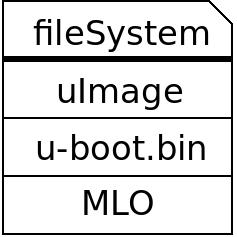
\includegraphics[scale=.4]{Imagenes/sd.jpg} 
  \end{center}
  \caption{Memoria SD}\label{Fig:HW} 
\end{figure}

En la FIGURA se pueden distinguir dos particiones, una en formato FAT32 y otra en formato ext3.
La partición con FAT32 es la partición de arranque en donde se encuentra el bootloader (MLO, u-boot.bin) y el kernel (uImage).
La partición con ext3 es la partición donde se encuentra el sistema de archivos (fileSystem).

El MLO es el equivalente bootloader de la primera etapa; en general ya viene precargado en la memoria NAND de la beagleboard. Es posible generarlo o incluso bajar una versión ya compilada desde la web de Angström. Como característica principal tiene la capacidad de buscar el u-boot.bin en dispositivos extraíbles como memorias SD o USB.

El u-boot.bin el equivalente al de la segunda etapa. Al igual que el MLO, es posible generarlo o incluso bajarlo de la web de Angström. En nuestro sistema fue necesario generarlo ya que configura el bloque de expansión de la beagleboard.

El uImage es el kernel del sistema. Fue necesario generarlo ya que se debieron modificar sus fuentes para que queden habilitadas las interfaces de comunicación con los dispositivos periféricos.

El fileSystem es el correspondiente a una distribución linux llamada Angström. Se pueden llegar a precargar distintos programas y bibliotecas dependiendo de la forma en que lo generemos.
Angström es una distribución linux diseñada específicamente para sistemas embebidos en microprocesadores como el nuestro. Esto lo hace más eficiente que otros sistemas operativos. La elección de esta distribución se debió a que es de los más recomendados y utilizados en la documentación y foros de Beagleboard.


\subsection{Bibliotecas}


\section{Herramientas utilizadas en el desarrollo del sistema}

\subsection{Introducción}
Para el desarrollo de sistemas, existe una gran variedad de herramientas útiles, algunas de software libre y otras privativas. El hecho de tener tantas opciones disponibles dificulta la elección de las herramientas. 

Para la elección de las herramientas tomamos como primer criterio de decisión el hecho de que sean libres y nos basamos en las experiencias de otras personas que ya han transitado caminos comunes, consultando y participando en foros activos.

A continuación se detallan las herramientas utilizadas para el desarrollo del sistema. 
Primero se da una descripción de las herramientas elegidas y luego EN se comentan otras que se probaron con igual o peor resultado que las herramientas elegidas en última instancia.

\subsection{Generación de MLO, u-boot.bin y uImage}
El MLO no fue necesario generarlo debido a su simpleza, ya que el binario precompilado realiza bien su función.

El u-boot.bin y el uImage fueron generados con la herramienta de desarrollo y compilación OpenEmbedded-Bitbake que es una fusión de dos herramientas: OpenEmbedded herramienta para construcción y mantenimiento de distribuciones y Bitbake herramienta de compilación similar al Make que automatiza la construcción de ejecutables entre otros. OpenEmbedded utiliza Bitbake para su objetivo. Es una herramienta muy potente y difícil de aprender al principio, luego de entendido su principio de funcionamiento se hace muy simple su utilización. Es necesaria una buena conexión a internet para su utilización.
Con esta herramienta también se pueden generar el MLO y el filesystem, aunque preferimos utilizar otras herramientas por sobre ésta. 
Su instalación, configuración, estructura y uso se pueden ver en el ANEXO. 


\subsection{Generación de FS}
Para la generación del fileSystem de Angström, se utilizó la herramienta web Narcissus.
Esta herramienta permite seleccionar entre diferentes dispositivos entre los cuales está beagleboard, los programas que se quieran instalar, el formato de la imágen seleccionada e incluso se puede generar un kit de desarrollo (SDK) para el host. Debido a la facildad de uso y a los buenos resultados obtenidos, se decidió utilizar esta opción por sobre la del filesystem generado por la herramienta OpenEmbedded-Bitbake.


\subsection{Croscompilación}
Para la croscompilación se utilizó el SDK generado por Narcissus y la herramienta Make para generar los archivos necesarios. La instalación el SDK se encuentra en el ANEXO.


\subsection{Depuración de código}
Para la depuración, se utilizó la herramienta GDB del proyecto GNU. 
Al momento de compilar, es necesario agregar la opción -g para que la aplicación pueda ser depurada. Esta opción agrega información en el código de la aplicación.
La interfaz del GDB es por consola, aunque existen algunos programas que utilizan GDB y además ofrecen una interfaz gráfica (DDD[referencia]).
Algunos de los comandos útiles y sus usos más comunes son: 

\bigskip
breakpoint: para colocar un breakpoint. En general se lo llama seguido del nombre de una función de la aplicación.

\bigskip
print: seguido del nombre de una variable, muestra el contenido de la variable durante el proceso de depuración. Si la variable es local a alguna función, el valor de la variable se pierde al salir de la función.

\bigskip
next: o “n”, sirve para ir línea a línea en modalidad step-over (sin entrar a las funciones).

\bigskip
step: o “s”, sirve para ir línea a línea en modalidad step-into (entrando a las funciones).

\bigskip
backtrace: o “bt”, despliega el stack de llamadas a funciones, sirve para saber por donde se pasó y donde estamos.

\bigskip
Sin olvidarnos del hecho de que la aplicación $RF^{2}$ está diseñada para una arquitectura distinta a la del PC de desarrollo, para el depurado de la aplicación existen dos alternativas. 

La primera es lo que se podría llamar depuración local, esto es, instalar GDB en la Beagleboard y depurar la aplicación en ésta. Para saber lo que sucede es necesario acceder de forma remota a ésta desde el PC de desarrollo. 

La segunda opción es la depuración remota. La depuración remota consiste en realizar la depuración de la aplicación desde el PC de desarrollo. Para esto, es necesario instalar GDBServer en la Beagleboard y tener instalado el GDB específico de la Beagleboard en el PC de desarrollo. Luego se establece una conexión que puede ser serial o ethernet entre la Beagleboard y el PC de desarrollo. Por más detalles sobre la configuración referirse al anexo.

\bigskip
La primera opción no es posible para sistemas embebidos chicos en los cuales no se puede instalar GDB, aunque éste no es el caso de la Beagleboard. 
Se tienen más y mejores herramientas en el PC de desarrollo, por ejemplo programas con interfaz gráfica que ayudan a entender mejor lo que está pasando. Por algunas de estas razones, se prefiere el uso de la depuración remota. 

\bigskip
Se utilizaron indistintamente tanto la primera opción como la segunda.

\subsection{Bibliotecas}

\section{Desarrollo}
\subsection{MLO}
\subsection{Multiplexado de pines}
El microprocesador OMAP3530 tiene muchos pines con distintas interfaces, pero no todas las 
señales son accecibles desde la BeagleBoard. Para poder acceder a las señales del microprocesador 
existe en la BeagleBoard un bloque de expansión de 28 pines. (dicho arriba)

Por defecto en el bloque de expansión no se encuentran las señales que nosotros queremos. Esto 
lleva a que se tenga que modificar el estado inicial de los pines. 
Existen dos formas de modificar los pines de modo que tengamos las señales que precisamos. Una 
de ellas es modificar el u-boot.bin, la otra es modificar el uImage (kernel). Cualquiera de estas modificaciones implica una compilación de los fuentes asociados al archivo en cuestión. 

Para la modificación de las señales disponibles en el bloque de expansión se decidió modificar el u- 
boot ya que la modificación por u-boot es más intuitiva y por experiencia sabemos que lo que más se actualiza y/o modifica es el kernel. 

\subsection{u-boot}
Como se mencionó anteriormente en el u-boot se realiza la configuración de los pines del bloque de expansión de la Beagleboard. “hacer referencia a tabla en algún lado”
Cada pin del bloque de expansión tiene varias funcionalidades asociadas, y la configuración de una 
funcionalidad depende de un multiplexado modificable a nivel de software. Esto es, dependiendo del “modo de pin” elegido, la señal que se obtiene en el pin.
Para que los cambios hechos en el u-boot tengan el efecto esperado al arrancar el sistema, es necesario que en la configuración del kernel esté la opción CONFIG\_OMAP\_MUX = no, ya que deshabilita posibles cambios en la configuración de los pines durante la carga del kernel. Esta opción no está activada por defecto en ninguna versión actual del kernel. 

Antes de modificar el estado de los pines del bloque de expansión es necesario obtener los fuentes del u-boot.

Nota: Puede que cuando se realiza la instalación de OpenEmbedded-Bitbake (anexooo), se genere un directorio relacionado con u-boot en /stuff/build/tmp/work/beagleboard-angstrom-linux-gnueabi/, si esto es así, no es necesario volver a obtener los fuentes.

Primero configuramos bitbake para poder utilizarlo:

\$ export BBPATH=/stuff/build:/stuff/openembedded

\$ export PATH=/stuff/bitbake/bin:\$PATH

Obtenemos los fuentes:

\$ cd /stuff/build

\$ bitbake -f -c clean -b ../openembedded/recipes/u-boot/u-boot\_git.bb

\$ bitbake -f -c compile -b ../openembedded/recipes/u-boot/u-boot\_git.bb

Los fuentes se encuentran en 

/stuff/build/tmp/work/beagleboard-angstrom-linux-gnueabi/u-boot.../git/.

En los fuentes del u-boot dentro de board/ti/beagle/ se encuentra el archivo beagle.h que es donde se establece la configuración de los pines del bloque de expansión de la beagleboard.

Si abrimos este archivo vamos a ver líneas del estilo: 
MUX\_VAL(CP(MCBSP3\_DX), (IEN | PTD | DIS | M4)) /*GPIO\_140*/$\backslash$ 

MUX\_VAL indica que se va a modificar el valor de multiplexado de lo que está entre paréntesis. 
CP(MCBSP3\_DX) es el Control\_PadConf, esto es el registro del microprocesador asociado con el 
pin a modificar. 
(IEN | PTD | DIS | M4) esta es la configuración del pin en cuestión: 

La opción IEN (input enable) hace que el pin sea bidireccional. 
La opción PTD y PTU, indica si el pin tiene un pull down o pull up respectivamente. 
La opción DIS y EN, indica si se deshabilitan o no las opciones PTD y PTU. 
La opción M4 es el modo seleccionado para del pin. Para la beagleboard existen 4 modos: M1, M2, M3 y M4.
GPIO\_140 es el nombre de la señal (ver que solo es un comentario). 

El Control\_PadConf es un registro de 32bits el cual controla el estado de dos pines, esto es, la parte 
baja del registro controla un pin y la parte alta controla otro. 

Analizando el “manual de referencia BeagleBoard del usuario” (“Expansion connector signals” – 
tabla 20), “manual técnico de referencia OMAP35x” (“SCM functional description” – capítulo 7.4) 
y agregando las opciones que nos interesan para los pines, se obtuvo la siguiente tabla: 

Al modificar el archivo beagle.h hay que tener mucho cuidado ya que al sustituir los valores no se deben repetir pines ni registros, no deben haber incoherencias, un registro por cada pin y un pin por cada registro. 
Dentro del archivo hay un macro definido MUX\_BEAGLE\_C(), donde se deben realizar las modificaciones ya que nuestro modelo de beagleboard es C4 y éste macro es el utilizado para este modelo de beagleboard.
En una primera instancia se sustituyeron los valores de la TABLA buscando los equivalentes del 
PadConf en el beagle.h. 

\#define MUX\_BEAGLE\_C() $\backslash$  

MUX\_VAL(CP(MCBSP3\_DX),	(IEN  | PTD | DIS | M4)) /*GPIO\_140*/$\backslash$  

MUX\_VAL(CP(MCBSP3\_DR),	(IEN  | PTD | DIS | M4)) /*GPIO\_142*/$\backslash$  

MUX\_VAL(CP(MCBSP3\_CLKX),	(IEN  | PTD | DIS | M4)) /*GPIO\_141*/$\backslash$  

MUX\_VAL(CP(MCBSP3\_FSX),	(IEN  | PTD | DIS | M1)) /*UART2\_RX*/$\backslash$  

MUX\_VAL(CP(UART2\_TX),		(IDIS | PTD | DIS | M0)) /*UART2\_TX*/$\backslash$  

MUX\_VAL(CP(MMC2\_DAT7),	(IEN  | PTD | EN  | M4)) /*GPIO\_139*/$\backslash$  

MUX\_VAL(CP(UART2\_CTS),	(IEN  | PTD | DIS | M4)) /*GPIO\_144*/$\backslash$  

MUX\_VAL(CP(MMC2\_DAT6),	(IEN  | PTD | EN  | M4)) /*GPIO\_138*/$\backslash$  

MUX\_VAL(CP(MMC2\_DAT5),	(IEN  | PTD | EN  | M4)) /*GPIO\_137*/$\backslash$  

MUX\_VAL(CP(MMC2\_DAT4),	(IEN  | PTD | EN  | M4)) /*GPIO\_136*/$\backslash$  

MUX\_VAL(CP(UART2\_RTS),	(IEN  | PTD | EN  | M4)) /*GPIO\_145*/$\backslash$  

MUX\_VAL(CP(MCBSP1\_DX),	(IEN  | PTD | EN  | M4)) /*GPIO\_158*/$\backslash$  

MUX\_VAL(CP(MMC2\_DAT2),	(IEN  | PTD | EN  | M4)) /*GPIO\_134*/$\backslash$  

MUX\_VAL(CP(MCBSP1\_CLKX),	(IEN  | PTD | EN  | M4)) /*GPIO\_162*/$\backslash$  

MUX\_VAL(CP(MMC2\_DAT1),	(IEN  | PTU | EN  | M4)) /*GPIO\_133*/$\backslash$  

MUX\_VAL(CP(MCBSP1\_FSX),	(IEN  | PTD | EN  | M4)) /*GPIO\_161*/$\backslash$  

MUX\_VAL(CP(MCBSP1\_DR),	(IEN  | PTD | EN  | M4)) /*GPIO\_159*/$\backslash$  

MUX\_VAL(CP(MCBSP1\_CLKR),	(IEN  | PTD | EN  | M4)) /*GPIO\_156*/$\backslash$  

MUX\_VAL(CP(MCBSP1\_FSR),	(IEN  | PTD | EN  | M4)) /*GPIO\_157*/$\backslash$  

MUX\_VAL(CP(I2C2\_SDA),		(IEN  | PTD | EN  | M4)) /*GPIO\_183*/$\backslash$  

MUX\_VAL(CP(I2C2\_SCL),		(IEN  | PTU | EN  | M4)) /*GPIO\_168*/$\backslash$  

MUX\_VAL(CP(MMC2\_DAT3),	(IEN  | PTD | EN  | M1)) /*SPI3\_CS0*/$\backslash$  

MUX\_VAL(CP(MMC2\_DAT0),	(IEN  | PTU | EN  | M1)) /*SPI3\_SOMI*/$\backslash$  

MUX\_VAL(CP(MMC2\_CMD),		(IEN  | PTU | DIS | M1)) /*SPI3\_SIMO*/$\backslash$  

MUX\_VAL(CP(MMC2\_CLK),		(IEN  | PTU | DIS | M1)) /*SPI3\_CLK*/


Luego es necesario compilar para obtener el u-boot.bin.

\$ cd /stuff/build

\$ bitbake -f -c compile -b ../openembedded/recipes/u-boot/u-boot\_git.bb

\$ bitbake -f -c deploy -b ../openembedded/recipes/u-boot/u-boot\_git.bb


Nota: Cada vez que introduzcamos un cambio, no es necesario ejecutar el comando con la opción clean (lo que implica volver a bajar los fuentes), solo basta con recompilar.

El archivo generado (u-boot.bin) se encuentra en 

/stuff/build/tmp/deploy/glibc/images/beagleboard/ aunque con su nombre seguido de un número identificatorio, el cual debe ser borrado para poder mantener el nombre u-boot.bin.

Pese a que en la literatura y foros, se plantea lo contrario, no fue posible establecer los atributos valor y dirección de los pines mediante la modificación planteada. Lo único que cambia es el modo del pin, con lo que se obtuvieron las señales que necesitamos. La solución a este inconveniente se muestra en (uImage-GPIO).


\subsection{uImage}
La versión del kernel elegida fue la 2.6.32 que en el momento del desarrollo era la versión más estable.(ver si en algún lado puse compatibilidad con distro) Aunque también se hicieron pruebas con las versiones 2.6.29 y 2.6.37 (pruebas!).
Durante la carga del uImage se cargan los módulos y controladores necesarios para funcionamiento del sistema embebido. También se montan las interfaces para poder interactuar con los distintos dispositivos a ser conectados a la Beagleboard como lo son: SPI, GPIO, UART, etc. Estas interfaces se deben encuentrar bajo /dev en el sistema operativo. En algunos casos, no aparecen algunas de las interfaces configuradas en /dev lo que lleva a modificar los fuentes del kernel para que esto así suceda. En el proyecto la interfaz SPI no quedó mapeada en /dev pese a que había sido configurada en el u-boot; también hubo problemas con los atributos valor y dirección de los GPIO comentado antes; y hacía falta un módulo para la conexión USB-ethernet con la cual conectar la Beagleboard con una PC como si fuera por red. Todo esto llevó a que se tuvieran que modificar los fuentes del uImage como se muestra a continuación:
 
Comando necesarios para el desarrollo del uImage:

\$ bitbake virtual/kernel -c comando

virtual/kernel: refiere a que estamos generando un kernel.

Entre los comandos:

clean: borra el contenido del directorio work. Borra todos los cambios hechos en la configuración del uImage fuente y parches agregados.

patch: genera los archivos de configuración y el fuente del uImage. Además le aplica los parches.

menuconfig: abre el editor de la configuración del kernel.

compile: compila todo.

deploy: genera los archivos referidos en este caso al uImage (.config, módulos, uImage) y los guarda en el directorio /stuff/build/tmp/deploy/glibc/images/beagleboard/.

Nota: Es necesario que todos estos comandos sean ejecutados en el orden adecuado para que todo funcione correctamente.

Primero configuramos bitbake para poder utilizarlo:

\$ export BBPATH=/stuff/build:/stuff/openembedded

\$ export PATH=/stuff/bitbake/bin:\$PATH

Comenzamos el desarrollo:

\$ cd /stuff/build

\$ bitbake virtual/kernel -c clean

\$ bitbake virtual/kernel -c patch

\$ bitbake virtual/kernel -c menuconfig


Luego de ejecutar este comando se abre el editor de la configuración del kernel (ver figura XXX). Es este editor es donde se indican qué módulos cargar y cuales no. En este caso un cambio de  configuración es necesario para el buen funcionamiento de la interfaz SPI y de la conexión USB-Ethernet con la Beagleboard.

\begin{figure}[H]
\centering
  \begin{center}
  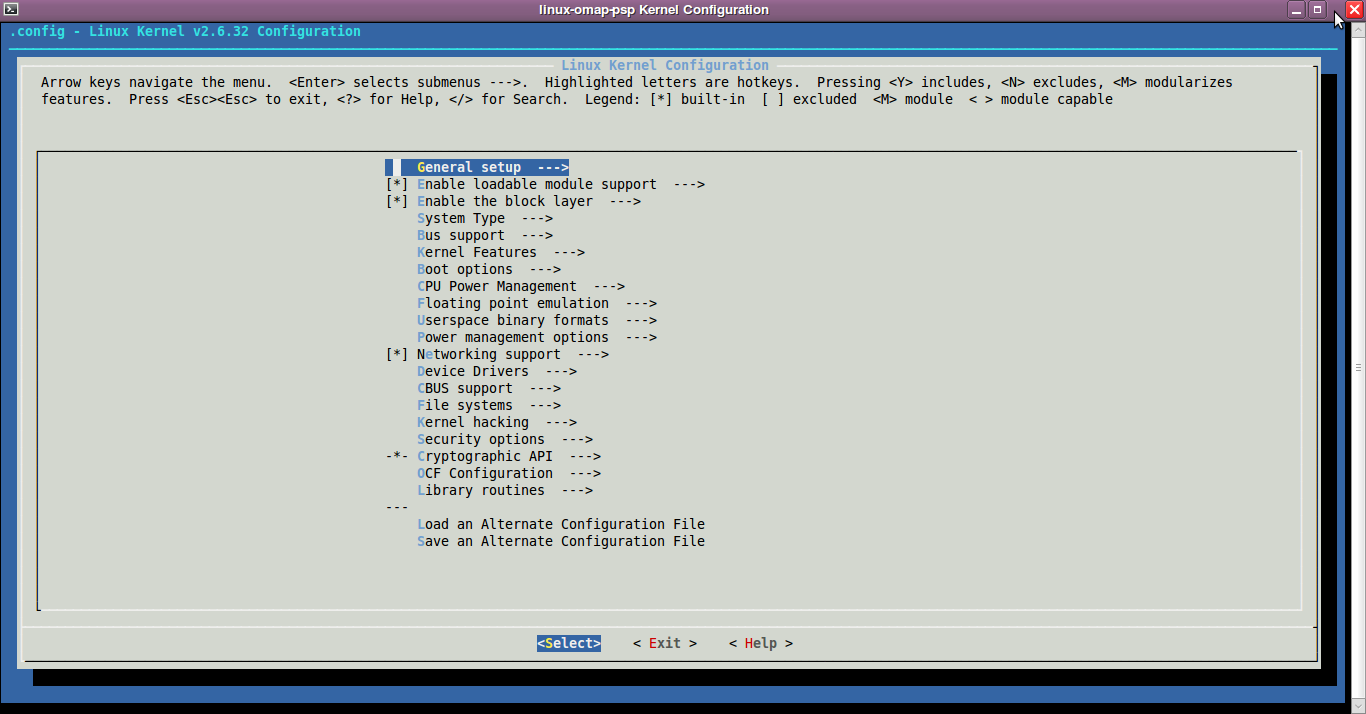
\includegraphics[scale=.3]{Imagenes/kernel.png} 
  \end{center}
  \caption{Editor de configuración del kernel}\label{Fig:HW} 
\end{figure}

Para configurar la interfaz SPI, se debe configurar como sigue:

Device Drivers – SPI Support=y y luego como en la figura XX.

\begin{figure}[H]
\centering
  \begin{center}
  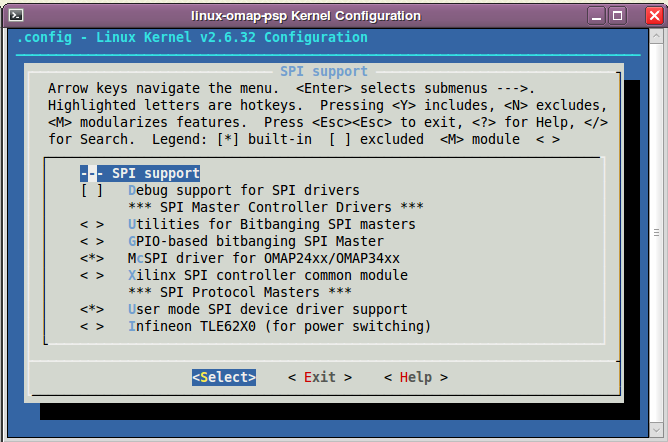
\includegraphics[scale=.4]{Imagenes/spi_chica.png} 
  \end{center}
  \caption{Configuración SPI}\label{Fig:HW} 
\end{figure}


Para poder establecer la conexión por USB con la Beagleboard, se debe configurar como sigue: 

Device Drivers – USB Support=y – USB Gadget Support=y y luego como en la figuraXX.

\begin{figure}[H]
\centering
  \begin{center}
  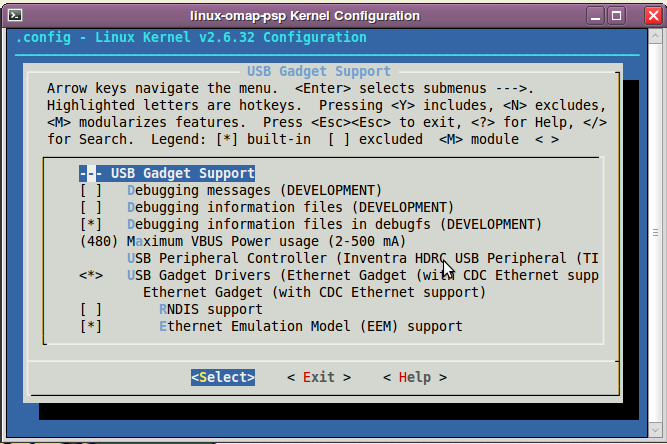
\includegraphics[scale=.4]{Imagenes/usb_chica.png} 
  \end{center}
  \caption{Configuración USB Gadget}\label{Fig:HW} 
\end{figure}

Luego, es necesario modificar el archivo board\_omap3beagle.c que se encuentra en /stuff/build/tmp/work/beagleboard-angstrom-linux-gnueabi/linux-omap-.../git/arch/arm/mach-omap2/. En este archivo está toda la inicialización de las interfaces. Los detalles de los cambios introducidos en este archivo se pueden obdervar en el anexo XXXX

Ahora se compila y genera el archivo uImage:

\$ bitbake virtual/kernel -c compile 

\$ bitbake virtual/kernel -c deploy 

Ahora dentro de /stuff/build/tmp/deploy/glibc/images/beagleboard/ está el archivo uImage generado.

Nota: Respecto al nombre del archivo, al igual que con el caso del u-boot.bin el nombre que aparece es un nombre más largo y necesita ser renombrado a uImage para que se pueda ejecutar correctamente.


\subsection{FileSystem}
\subsection{Bibliotecas}


\section{Ejecución de programa principal}
\subsection{Script para ejecución autónoma}
